\documentclass[aspectratio=169]{beamer}

% Pakete laden
% Paket für Deutsche Sprache (Übersetzungen von Chapter zu Kapitel, 
% richtige Umlaute, richtige % Silbentrennung)
% siehe auch http://de.wikipedia.org/wiki/Babel-System
\usepackage[english]{babel}

% Ausgabeschriftart von LaTeX festlegen
\usepackage[T1]{fontenc}

% Standardpfad für Grafiken
\graphicspath{{logos/}{bilder/}{../root/}{../figures/}}

% Paket zum Erstellen von Plots mit TikZ
\usepackage{pgfplots}
% immer die neueste Version benutzen
\pgfplotsset{compat=newest}
% Verbindung von Linien durch eine schräge Kante
\pgfplotsset{every axis/.append style={line join=bevel}}
% Formatvorlage für Präsentationen
\mode<beamer>{
	\pgfplotsset{
		beamer/.style={
			width=0.8\textwidth,
			height=0.45\textwidth,
			legend style={font=\scriptsize},
			tick label style={font=\footnotesize},
			label style={font=\small},
			max space between ticks=28,
		}
	}
}
\mode<handout>{
	\pgfplotsset{
		beamer/.style={
			width=0.8\textwidth,
			height=0.45\textwidth,
			legend style={font=\scriptsize},
			tick label style={font=\footnotesize},
			label style={font=\small},
			max space between ticks=25,
		}
	}
}
\mode<article>{
	\pgfplotsset{
		beamer/.style={
			width=0.8\textwidth,
			height=0.45\textwidth,
			max space between ticks=35,
		}
	}
}
% neue Größenvorlage für zwei Plots nebeneinander anlegen
\pgfplotsset{
	scriptsize/.style={
		width=0.34\textwidth,
		height=0.1768\textwidth,
		legend style={font=\scriptsize},
		tick label style={font=\scriptsize},
		label style={font=\footnotesize},
		title style={font=\footnotesize},
		every axis title shift=0pt,
		max space between ticks=25,
		every mark/.append style={mark size=7},
		major tick length=0.1cm,
		minor tick length=0.066cm,
	}
}
\pgfplotsset{
	small/.style={
		width=6.5cm,
		height=,
		tick label style={font=\footnotesize},
		label style={font=\small},
		legend style={font=\footnotesize},
		max space between ticks=30,
	}
}
% Legendeneintrage standardmäßig links ausrichten
\pgfplotsset{legend cell align=left}
% Hauptgitternetz zeichnen
\pgfplotsset{xmajorgrids}
\pgfplotsset{ymajorgrids}
% Anzahl der kleinen Teilstriche zwischen zwei großen Teilstrichen
%\pgfplotsset{minor x tick num={3}}
%\pgfplotsset{minor y tick num={3}}
% feines Gitternetz zeichnen
%\pgfplotsset{xminorgrids}
%\pgfplotsset{yminorgrids}
% nur nach den Achsen skalieren
\pgfplotsset{scale only axis}
% Farben wie in MATLAB definieren
\definecolor{matlab1}{rgb}{0,0,1}
\definecolor{matlab2}{rgb}{0,0.5,0}
\definecolor{matlab3}{rgb}{1,0,0}
\definecolor{matlab4}{rgb}{0,0.75,0.75}
\definecolor{matlab5}{rgb}{0.75,0,0.75}
\definecolor{matlab6}{rgb}{0.75,0.75,0}
\definecolor{matlab7}{rgb}{0.25,0.25,0.25}
% Farbreihenfolge wie in MATLAB definieren
\pgfplotscreateplotcyclelist{matlab}{
	{matlab1,solid},
	{matlab2,dashed},
	{matlab3,dashdotted},
	{matlab4,dotted},
	{matlab5,densely dashed},
	{matlab6,densely dashdotted},
	{matlab7,densely dotted}% dies unterdrückt einen Fehler
}
% Farbreihenfolge wie in MATLAB benutzen
\pgfplotsset{cycle list name=matlab}
% Farbreihenfolge von pgfplots benutzen
%\pgfplotsset{cycle list name=color list}
% nur Graustufen benutzen
%\pgfplotsset{cycle list name=linestyles}
% Strichstärke auf 1pt festlegen
\pgfplotsset{every axis plot/.append style={line width=1pt}}
% für deutsche Dokumente ein Komma benutzen
\addto\extrasngerman{\pgfplotsset{/pgf/number format/.cd,set decimal separator={{{,}}}}}
% ein halbes Leerzeichen als Tausendertrennzeichen benutzen
%\pgfplotsset{/pgf/number format/.cd,1000 sep={\,}}
% kein Tausendertrennzeichen verwenden
\pgfplotsset{/pgf/number format/.cd,1000 sep={}}
% Zahlen kleiner als 0.1 auch im fixed-Format ausgeben
\pgfplotsset{/pgf/number format/.cd,std=-2}
% neue Positionen für Legenden anlegen
\pgfplotsset{/pgfplots/legend pos/north/.style={/pgfplots/legend style={at={(0.50,0.97)},anchor=north}}}
\pgfplotsset{/pgfplots/legend pos/south/.style={/pgfplots/legend style={at={(0.50,0.03)},anchor=south}}}
\pgfplotsset{/pgfplots/legend pos/east/.style={/pgfplots/legend style={at={(0.97,0.50)},anchor=east}}}
\pgfplotsset{/pgfplots/legend pos/west/.style={/pgfplots/legend style={at={(0.03,0.50)},anchor=west}}}
\pgfplotsset{/pgfplots/legend pos/outer north/.style={/pgfplots/legend style={at={(0.50,1.03)},anchor=south}}}

% Paket für SI-Einheiten
\usepackage{siunitx}
% Brüche aktivieren
\sisetup{per-mode=fraction}
% Dezimaltrennzeichen abhängig von der Sprache
\addto\extrasngerman{\sisetup{output-decimal-marker={,}}}
\addto\extrasenglish{\sisetup{output-decimal-marker={.}}}
% Trennzeichen für Bereiche
\addto\extrasngerman{\sisetup{range-phrase={ bis~}}} 
\addto\extrasenglish{\sisetup{range-phrase={ to~}}}

% Paket, um das Floating in Article-Modus abzuschalten
\usepackage{float}

% Paket, um anderen Zeilenabstand einzustellen, besonders für Tabellen
\usepackage{setspace}

% Paket für ein intelligentes Leerzeichen
\usepackage{xspace}

% Abkürzung für z. B.
\newcommand{\zB}{z.\,B.\xspace}

% Paket für schönere Brüche im Textmodus
\usepackage{xfrac}

% schönere Tabellen
\usepackage{booktabs}

% schönere Anführungszeichen
\usepackage{csquotes}

% Labeling-Umgebung definieren
\makeatletter
\newenvironment{labeling}[2][]{%
  \def\sc@septext{#1}%
  \list{}{\settowidth{\labelwidth}{{%
        #2%
          \sc@septext%
      }}%
    \leftmargin\labelwidth \advance\leftmargin by \labelsep
    \let\makelabel\labelinglabel
  }%
}{%
  \endlist
}
\newcommand\labelinglabel[1]{%
  #1\hfil
    \sc@septext%
}
\makeatother

% BibLaTeX-Paket für Zitate
\usepackage[%
	style=ieee,%				format wie beim IEEE
	backend=biber,%			Warnung unterdrücken
]{biblatex}

% Datenbank der Literaturquellen
\addbibresource{literatur.bib}

% Paket zur Darstellung von QR-Codes
\usepackage{qrcode}

% Wie entfernt man einige Seiten aus den Navigationspunkten in Beamer?
% see: https://tex.stackexchange.com/questions/37127/how-to-remove-some-pages-from-the-navigation-bullets-in-beamer
\makeatletter
\let\beamer@writeslidentry@miniframeson=\beamer@writeslidentry
\def\beamer@writeslidentry@miniframesoff{%
	\expandafter\beamer@ifempty\expandafter{\beamer@framestartpage}{}% does not happen normally
	{%else
		% removed \addtocontents commands
		\clearpage\beamer@notesactions%
	}
}
\newcommand*{\miniframeson}{\let\beamer@writeslidentry=\beamer@writeslidentry@miniframeson}
\newcommand*{\miniframesoff}{\let\beamer@writeslidentry=\beamer@writeslidentry@miniframesoff}
\makeatother

% Abstand zwischen den Punkten von subsections in der Miniframe-Navigation
% siehe: http://tex.stackexchange.com/questions/288548/beamer-miniframes-horizontal-space-between-dots-when-using-the-compress-option
\makeatletter
\def\slideentry#1#2#3#4#5#6{%
  %section number, subsection number, slide number, first/last frame, page number, part number
  \ifnum#6=\c@part\ifnum#2>0\ifnum#3>0%
    \ifbeamer@compress%
      \advance\beamer@xpos by1\relax%
      \ifnum1=#3                        %%% NOTICE
				\ifnum1=#2\else
					\advance\beamer@xpos by1\relax% %%% THESE
				\fi
      \fi                               %%% LINE
    \else%
      \beamer@xpos=#3\relax%
      \beamer@ypos=#2\relax%
    \fi%
  \hbox to 0pt{%
    \beamer@tempdim=-\beamer@vboxoffset%
    \advance\beamer@tempdim by-\beamer@boxsize%
    \multiply\beamer@tempdim by\beamer@ypos%
    \advance\beamer@tempdim by -.05cm%
    \raise\beamer@tempdim\hbox{%
      \beamer@tempdim=\beamer@boxsize%
      \multiply\beamer@tempdim by\beamer@xpos%
      \advance\beamer@tempdim by -\beamer@boxsize%
      \advance\beamer@tempdim by 1pt%
      \kern\beamer@tempdim
      \global\beamer@section@min@dim\beamer@tempdim
      \hbox{\beamer@link(#4){%
          \usebeamerfont{mini frame}%
          \ifnum\c@section=#1%
            \ifnum\c@subsection=#2%
              \usebeamercolor[fg]{mini frame}%
              \ifnum\c@subsectionslide=#3%
                \usebeamertemplate{mini frame}%\beamer@minislidehilight%
              \else%
                \usebeamertemplate{mini frame in current subsection}%\beamer@minisliderowhilight%
              \fi%
            \else%
              \usebeamercolor{mini frame}%
              %\color{fg!50!bg}%
              \usebeamertemplate{mini frame in other subsection}%\beamer@minislide%
            \fi%
          \else%
            \usebeamercolor{mini frame}%
            %\color{fg!50!bg}%
            \usebeamertemplate{mini frame in other subsection}%\beamer@minislide%
          \fi%
        }}}\hskip-10cm plus 1fil%
  }\fi\fi%
  \else%
  \fakeslideentry{#1}{#2}{#3}{#4}{#5}{#6}%
  \fi\ignorespaces
}


% IIT Indore Beamer Theme
\usepackage{beamer_iiti}

% Metadata
\title[Machine Learning in Forex]{Machine Learning in Forex}
\subtitle{Literature Review and Baseline Models}
\author[Prince Kumar]{%
  \textbf{Prince Kumar} (Roll No. 230051013)\\[0.5em]
  \small \textbf{Supervisors:} Prof. Raghunath Sahoo \& Dr. Kalindi C. Pradhan
}
\institute[IIT Indore]{
  \textbf{Department of Physics}\\
  \textbf{Indian Institute of Technology Indore}
}
\date{\today}

\begin{document}

%----------------------------------------------------------------------------------------
% TITLE PAGE
%----------------------------------------------------------------------------------------
\begin{withoutheadline}
\begin{frame}[plain]
	\titlepage
\end{frame}
\end{withoutheadline}

%----------------------------------------------------------------------------------------
% OUTLINE PAGE
%----------------------------------------------------------------------------------------
\begin{frame}[label=inhalt]{Presentation Agenda}
	\tableofcontents
\end{frame}

%========================================================================================
\section{Introduction \& Objectives}
%========================================================================================
\subsection*{}

\begin{frame}{Background \& Research Motivation}
	\begin{block}{Foreign Exchange (Forex) Dynamics}
		\begin{itemize}
			\item \textbf{Volatility \& Non-Stationarity:} Currency markets exhibit non-linear interactions, microstructural noise, and macro-economic regime shifts.
			\item \textbf{Transition in Predictive Modeling:} Evolution from rule-based technical analysis to Deep Learning (DL), Recurrent Networks (LSTM), and Reinforcement Learning (RL).
		\end{itemize}
	\end{block}

\end{frame}

\begin{frame}{Background \& Research Motivation}

	\begin{block}{The Dual Goal of This Work}
		\begin{itemize}
			\item \textbf{Literature Survey:} Critically examine representative machine learning and deep learning methodologies for foreign-exchange forecasting.
			\item \textbf{Transparent Reference Baseline:} Implement and benchmark a reproducible, next-day continuous exchange-rate forecasting framework on USD/INR.
		\end{itemize}
	\end{block}
\end{frame}

\begin{frame}{Free-Floating vs Managed Currency Dynamics}
	\begin{block}{Why Models Work Better on EUR/USD Than USD/INR}
		It was noticed that literature shows higher accuracy and profits on \textbf{EUR/USD} than \textbf{USD/INR}. This stems from fundamentally different market regimes:
	\end{block}
\end{frame}

\begin{frame}{Free-Floating vs Managed Currency Dynamics}
	
	\begin{columns}[T]
		\begin{column}{0.48\textwidth}
			\begin{block}{Free-Floating Regime (EUR/USD)}
				\begin{itemize}
					\item \textbf{Pure Market Mechanics:} High liquidity, market-driven order flow, unconstrained price discovery.
					\item \textbf{Predictable Technical Signals:} Price moves reflect macroeconomic expectations and technical indicator patterns.
				\end{itemize}
			\end{block}
		\end{column}
		\begin{column}{0.48\textwidth}
			\begin{block}{Managed Float Regime (USD/INR)}
				\begin{itemize}
					\item \textbf{RBI Central Bank Interventions:} The Reserve Bank of India (RBI) actively intervenes (dollar buying/selling, repo operations, LAF) to suppress volatility.
					\item \textbf{Exogenous Shocks:} Artificial price stabilization introduces non-market regime shifts, degrading standard ML model performance.
				\end{itemize}
			\end{block}
		\end{column}
	\end{columns}
\end{frame}

\begin{frame}{Problem Formulation: Point Prediction vs Classification}
	\begin{block}{Target Definition}
		Let $C_t$ denote the USD/INR exchange rate on day $t$. The model directly predicts the continuous next-day price:
		\begin{equation}
			y_t = C_{t+1} \quad \text{or next log return } r_{t+1} = \ln(C_{t+1}/C_t)
		\end{equation}
	\end{block}
\end{frame}

\begin{frame}{Problem Formulation: Point Prediction vs Classification}

	\begin{block}{Key Methodological Advantages}
		\begin{itemize}
			\item \textbf{Decoupled Regression:} Training minimizes Mean Squared Error (MSE), avoiding loss of magnitude information inherent in discrete labels.
			\item \textbf{Post-Hoc Directional Metric:} Directional accuracy is calculated post-hoc by evaluating $\text{sign}(\hat{y}_t - C_t)$.
			\item \textbf{Benchmark Standard:} Provides a rigorous point-prediction baseline before adding action-selection or reinforcement learning layers.
		\end{itemize}
	\end{block}
\end{frame}

%========================================================================================
\section{Literature Review}
%========================================================================================
\subsection*{}

\begin{frame}{Overview of Reviewed Literature}
	
	\begin{columns}[T]
		\begin{column}{0.48\textwidth}
			\begin{itemize}
				\item \textbf{1. FOREX Trend (2011):} SVM, MLP, RBF + GARCH, PCA, LDA, MCML, NCA.
				\item \textbf{2. Deep TA (2021):} ResNet50, ViT on candlestick charts + GA rules.
				\item \textbf{3. Financial DRQN (2018):} DRQN + Action Augmentation across 12 pairs.
				\item \textbf{4. Macro-Quant (2025):} XGBoost + SHAP for 5-day USD/INR prediction.
			\end{itemize}
		\end{column}
		\begin{column}{0.48\textwidth}
			\begin{itemize}
				\item \textbf{5. LSTM + RL (2019):} 2-layer LSTM + RL Motor Map for HFT trend correction.
				\item \textbf{6. AlgoML (2022):} Ensemble (DQN, PPO, BiLSTM) + GA Pullback strategy.
				\item \textbf{7. Adaptive RRL (2006):} Recurrent RL + Dynamic Utility Optimization.
				\item \textbf{8. Macro Interpretive (2023):} LASSO, Ridge, XGBoost, LGBM, GRU + SHAP on CAD/USD.
			\end{itemize}
		\end{column}
	\end{columns}
\end{frame}

\begin{frame}{Literature Review Summary (1/2)}
	\resizebox{\textwidth}{!}{%
	\begin{tabular}{cllllll p{3.5cm}}
		\toprule
		\textbf{\#} & \textbf{Paper} & \textbf{Year} & \textbf{Target / Task} & \textbf{Market / Data} & \textbf{Model / Architecture} & \textbf{Evaluation} & \textbf{Key Results} \\
		\midrule
		\textbf{1} & FOREX Trend Classification & 2011 & Binary: Next-day High/Low & USD/JPY, EUR/EGP (OHLCV) & SVM, MLP, RBF, PCA, LDA, MCML, NCA & Accuracy, PNP & Best accuracy 79.8\% (EUR/SAR); best PNP 67.7\% (EUR/EGP). \\
		\midrule
		\textbf{2} & Can Deep Learning Improve TA? & 2021 & Classification: Buy/Sell/Stay & GBP/USD, EUR/USD (MetaTrader) & ResNet50, ViT + GA + Simulation & Net Profit, Sharpe, Drawdown & ~20.2\% avg gain; AI deep learning rule itself did not learn effective policy. \\
		\midrule
		\textbf{3} & Financial Trading as a Game & 2018 & Decision: Long/Neutral/Short & 12 Forex pairs (TrueFX ticks) & Financial DRQN + Action Augmentation & Annual Return, Sharpe, MDD & Positive returns for all 12 pairs. \\
		\midrule
		\textbf{4} & Macro-Quant (USD/INR) & 2025 & 5-day Direction: Up/Down & USD/INR (Yahoo + FRED) & XGBoost + Stationarity + SHAP & Accuracy, Sharpe, Net Return & 60.96\% accuracy vs 50\% random walk; trading strategy produced $-16\%$ return. \\
		\bottomrule
	\end{tabular}%
	}
\end{frame}

\begin{frame}{Literature Review Summary (2/2)}
	\resizebox{\textwidth}{!}{%
	\begin{tabular}{cllllll p{3.5cm}}
		\toprule
		\textbf{\#} & \textbf{Paper} & \textbf{Year} & \textbf{Target / Task} & \textbf{Market / Data} & \textbf{Model / Architecture} & \textbf{Evaluation} & \textbf{Key Results} \\
		\midrule
		\textbf{5} & Deep LSTM with RL Layer & 2019 & Trend: SHORT/LONG/Range & EUR/USD, EUR/GBP (Tickstory) & 2-layer LSTM + RL Motor Map & Accuracy, ROI, Max Drawdown & LSTM alone ~70\%; adding RL reached ~85\% accuracy, 98.23\% ROI, 15.97\% MD. \\
		\midrule
		\textbf{6} & AlgoML Ensemble & 2022 & Next-day Buy/Sell Signal & EUR/USD (OANDA data) & Ensemble (DQN, PPO, BiLSTM) + GA Pullback & Accuracy, P\&L, Max Drawdown & Ensemble: 9.97\% P\&L; GA Pullback strategy: 10.55\% P\&L. \\
		\midrule
		\textbf{7} & Adaptive RL System & 2006 & Signal: Long vs Short & EUR/USD 1-min (HSBC Bank) & Recurrent RL (RRL) + Dynamic Utility & Profit, Pips, Utility, Drawdown & 5,104 pips (~26\% p.a.) vs $-1,636$ pips for Buy-and-Hold; 61--63\% direction. \\
		\midrule
		\textbf{8} & Macro Interpretive ML & 2023 & Rate Forecasting (1, 5, 10-step) & CAD/USD (Bank of Canada, FRED) & LASSO, Ridge, XGB, LGBM, GRU + SHAP & NRMSE, MAE, SHAP Importance & LASSO best for 1-day; LGBM best for 1-week; XGB best long-horizon; GRU weaker. \\
		\bottomrule
	\end{tabular}%
	}
\end{frame}

%----------------------------------------------------------------------------------------
% DETAILED PAPER BREAKDOWNS (FROM HANDWRITTEN NOTES & RECENT PAPERS)
%----------------------------------------------------------------------------------------

\begin{frame}{Deep Dive: Feature Extraction \& Dimensionality Reduction (2011)}
	\begin{block}{Input Feature Representation (81 Features)}
		Combines 46 Technical Analysis (TA) parameters, 2 GARCH volatility estimates, and signal processing features (averages, slopes, Fourier components, sine terms).
	\end{block}
	
\end{frame}

\begin{frame}{Deep Dive: Feature Extraction \& Dimensionality Reduction (2011)}
	
	\begin{columns}[T]
		\begin{column}{0.48\textwidth}
			\begin{block}{Class-Based Metric Learning}
				\begin{itemize}
					\item \textbf{PCA:} 2D PCA transformations computed separately on UP and DOWN trends to preserve directional variance.
					\item \textbf{MCML:} Maximally Collapsing Metric Learning maps intra-class samples to single points in feature space.
					\item \textbf{NCA:} Neighborhood Components Analysis clusters multivariate data using distance metrics.
				\end{itemize}
			\end{block}
		\end{column}
		\begin{column}{0.48\textwidth}
			\begin{block}{Cluster-LDA Feature Generation}
				K-Means separates UP ($U_1,U_2,U_3$) and DOWN ($D_1,D_2,D_3$) clusters:
				\begin{itemize}
					\item \textbf{Cluster-Class LDA:} Compares $D_i$ vs All UP ($2 \times k = 6$ features).
					\item \textbf{Cluster-Cluster LDA:} Compares $U_i$ vs $D_j$ ($k^2 = 9$ features).
					\item Yields 15 pattern features for classifiers (SVM, MLP, RBF).
				\end{itemize}
			\end{block}
		\end{column}
	\end{columns}
\end{frame}

\begin{frame}{Deep Dive: Feature Extraction \& Dimensionality Reduction (2011)}
	
	\begin{columns}[T]
		\begin{column}{0.48\textwidth}
			\begin{block}{Class-Based Metric Learning}
				\begin{itemize}
					\item \textbf{NCA:} Neighborhood Components Analysis clusters multivariate data using distance metrics.
				\end{itemize}
			\end{block}
		\end{column}
		\begin{column}{0.48\textwidth}
			\begin{block}{Cluster-LDA Feature Generation}
				K-Means separates UP ($U_1,U_2,U_3$) and DOWN ($D_1,D_2,D_3$) clusters:
				\begin{itemize}
					\item \textbf{Cluster-Class LDA:} Compares $D_i$ vs All UP ($2 \times k = 6$ features).
					\item \textbf{Cluster-Cluster LDA:} Compares $U_i$ vs $D_j$ ($k^2 = 9$ features).
					\item Yields 15 pattern features for classifiers (SVM, MLP, RBF).
				\end{itemize}
			\end{block}
		\end{column}
	\end{columns}
\end{frame}

\begin{frame}{Deep Dive: Technical Analysis \& Genetic Optimization (2021)}
	\begin{block}{Price Filtering: Modified Renko Bars}
		Replaces fixed time intervals with price movement thresholds. A new brick forms only when price moves by brick size, eliminating microstructural noise and yielding 20--200\% strategy returns.
	\end{block}

\end{frame}

\begin{frame}{Deep Dive: Technical Analysis \& Genetic Optimization (2021)}

	\begin{columns}[T]
		\begin{column}{0.48\textwidth}
			\begin{block}{Donchian Channels \& Vision Models}
				\begin{itemize}
					\item \textbf{Donchian Channel:} Upper band (highest high), Lower band (lowest low), Middle band (average).
					\item \textbf{Vision Models:} ResNet50 (CNN) and Vision Transformer (ViT) on candlestick images.
				\end{itemize}
			\end{block}
		\end{column}
		\begin{column}{0.48\textwidth}
			\begin{block}{Two-Phase GA \& Critical Finding}
				\begin{itemize}
					\item \textbf{Genetic Algorithm:} Chromosomes encode TA indicators and AI rules via mutation/crossover.
					\item \textbf{Critical Finding:} AI-generated rules were discarded in Phase 2 trading simulation because they failed to improve upon pure TA rules.
				\end{itemize}
			\end{block}
		\end{column}
	\end{columns}
\end{frame}

\begin{frame}{Deep Dive: Deep RL \& Portfolio MDP Dynamics (2018)}
	\begin{block}{Markov Decision Process (MDP) \& Logarithmic Rewards}
		State-based reward calculation independent of history: $G_t = R_{t+1} + \gamma R_{t+2} + \gamma^2 R_{t+3} + \dots$
		$$\text{Additive Logarithmic Reward: } r_t = \log \left(\frac{N_t}{N_{t-1}}\right)$$
		where $N_t = N_{t-1} + a_t \cdot c \cdot (C_t - O_t) - d_t$ is portfolio value, $a_t \in \{-1,0,+1\}$, $c$ trade size, $d_t$ spread cost.
	\end{block}

\end{frame}

\begin{frame}{Deep Dive: Deep RL \& Portfolio MDP Dynamics (2018)}

	\begin{columns}[T]
		\begin{column}{0.48\textwidth}
			\begin{block}{DRQN Architecture ($\sim 65\text{k}$ Parameters)}
				\begin{itemize}
					\item Input $\to$ 256 units $\to$ ELU $\to$ 256 units $\to$ LSTM $\to$ Linear output (3 actions).
					\item \textbf{Weight Init:} Biases $\approx 0$, forget gate $= 1$, output weights $\approx$ tiny random values.
				\end{itemize}
			\end{block}
		\end{column}
		\begin{column}{0.48\textwidth}
			\begin{block}{Features \& Empirical Performance}
				\begin{itemize}
					\item \textbf{Inputs:} Sinusoidal time encodings $\sin(2\pi t/T)$, $16 \times 12$ market features, position state $\mathbb{R}^3$.
					\item \textbf{Results:} Positive returns across 12 pairs (9.5\% EUR/USD to 60.8\% CHF/JPY).
				\end{itemize}
			\end{block}
		\end{column}
	\end{columns}
\end{frame}


\begin{frame}{Deep Dive: Macroeconomic Fundamentals \& Interpretive ML (2023)}
	\begin{block}{CAD/USD Exchange Rate Forecasting via Macro Fundamentals}
		Evaluates multi-horizon forecasting (1, 5, 10 steps ahead) using macroeconomic factors (Oil, Gold, TSX, S\&P 500, Eurodollar rate, interest rate differential, PPI, M1, Unemployment, Industrial Production).
	\end{block}

\end{frame}

\begin{frame}{Deep Dive: Macroeconomic Fundamentals \& Interpretive ML (2023)}

	\begin{columns}[T]
		\begin{column}{0.48\textwidth}
			\begin{block}{Model Spectrum \& SHAP Interpretability}
				\begin{itemize}
					\item \textbf{Linear Regularized:} LASSO, Ridge.
					\item \textbf{Tree Ensembles:} Extra Trees, XGBoost, LightGBM.
					\item \textbf{Recurrent Neural Net:} GRU.
					\item \textbf{SHAP Feature Attribution:} Identifies macroeconomic drivers across economic regimes.
				\end{itemize}
			\end{block}
		\end{column}
		\begin{column}{0.48\textwidth}
			\begin{block}{Key Empirical Insights}
				\begin{itemize}
					\item \textbf{Short Horizon (1-day):} Regularized linear models (LASSO) performed best.
					\item \textbf{Medium Horizon (1-week):} LightGBM achieved superior NRMSE/MAE.
					\item \textbf{Long Horizon (10-day):} XGBoost dominated; GRU showed weaker generalization.
				\end{itemize}
			\end{block}
		\end{column}
	\end{columns}
\end{frame}

\begin{frame}{Identified Research Gap: Post-Hoc Analysis of Macro Features on RL Models}

	\begin{columns}[T]
		\begin{column}{0.48\textwidth}
			\begin{block}{Reinforcement Learning Studies}
				\begin{itemize}
					\item Focus on price/technical inputs and trading execution (DRQN, AlgoML, Adaptive RRL).
					\item \textbf{Limitation:} Treat RL policies as "black boxes" without explaining how individual macro features drive action selection ($Q(s,a)$).
				\end{itemize}
			\end{block}
		\end{column}
		\begin{column}{0.48\textwidth}
			\begin{block}{Macroeconomic ML Studies}
				\begin{itemize}
					\item Use macroeconomic factors + SHAP explainability (Macro-Quant 2025, CAD/USD 2023).
					\item \textbf{Limitation:} Restricted to static classification / regression (XGBoost/LASSO), lacking dynamic RL portfolio execution.
				\end{itemize}
			\end{block}
		\end{column}
	\end{columns}

\end{frame}

\begin{frame}{Identified Research Gap: Post-Hoc Analysis of Macro Features on RL Models}

	\begin{center}
		\small \textbf{Core Research Gap:} Applying \textbf{Post-Hoc SHAP Analysis} to evaluate the impact of \textbf{Macroeconomic Features \& Differentials} on \textbf{Reinforcement Learning Policies} under managed float (RBI) regimes.
	\end{center}
\end{frame}

%========================================================================================
\section{Dataset \& Feature Engineering}
%========================================================================================
\subsection*{}

\begin{frame}{Comprehensive Feature Space Breakdown}
	\begin{block}{Core FX \& Macro Interest Rates}
		\textbf{\texttt{DEXINUS}} (USD/INR Target), \textbf{\texttt{jpy}} (USD/JPY), \textbf{\texttt{eur}} (EUR/USD), \textbf{\texttt{repo\_rate}} (RBI Repo Rate / FFER), \textbf{\texttt{treasury\_yield}} (10-Yr US Treasury Yield).
	\end{block}
\end{frame}

\begin{frame}{Comprehensive Feature Space Breakdown}

	\begin{columns}[T]
		\begin{column}{0.48\textwidth}
			\begin{block}{Global Commodities}
				\begin{itemize}
					\item \textbf{Precious Metals:} \texttt{gold}, \texttt{silver}
					\item \textbf{Energy:} \texttt{wti\_crude}, \texttt{brent\_crude}
					\item \textbf{Industrial Metals:} \texttt{copper}, \texttt{aluminium}, \texttt{zinc}, \texttt{nickel}
				\end{itemize}
			\end{block}
			\begin{block}{US Market Features}
				\begin{itemize}
					\item \textbf{\texttt{sp500\_close}}, \textbf{\texttt{sp500\_volume}}
				\end{itemize}
			\end{block}
		\end{column}
		\begin{column}{0.48\textwidth}
			\begin{block}{India Domestic Market Features}
				\begin{itemize}
					\item \textbf{Volatility \& Equities:} \texttt{india\_vix\_close}, \texttt{nifty50\_close}, \texttt{niftybank\_close}
					\item \textbf{Valuation Fundamentals:} \texttt{nifty50\_pe}, \texttt{nifty50\_pb}, \texttt{nifty50\_div\_yield}, \texttt{niftybank\_pe}, \texttt{niftybank\_pb}, \texttt{niftybank\_div\_yield}
					\item \textbf{Domestic Gold:} \texttt{india\_gold}
				\end{itemize}
			\end{block}
		\end{column}
	\end{columns}
\end{frame}

\begin{frame}{Proposed Novel Features: Macroeconomic Differentials \& Spreads}

	\begin{columns}[T]
		\begin{column}{0.48\textwidth}
			\begin{block}{Interest Rate \& Yield Spreads}
				\begin{itemize}
					\item \textbf{Rate of Change Features:}
						\[
						\operatorname{ROC}_k(x_t) =
						100\left(\frac{x_t}{x_{t-k}} - 1\right)
						\]
					\item Applied to VIX, interest rates, and yields for $k=1$ and $k=5$ days.
				\end{itemize}
			\end{block}
		\end{column}
		\begin{column}{0.48\textwidth}
			\begin{block}{Commodity \& Equity Differentials}
				\begin{itemize}
					\item \textbf{Returns and Relative Changes:}
						\[
						r_t(x) = \frac{x_t}{x_{t-1}} - 1,
						\qquad
						\Delta\log x_t = \log x_t - \log x_{t-1}
						\]
					\item Applied to commodities, equities, FX, and India--US price ratios.
				\end{itemize}
			\end{block}
		\end{column}
	\end{columns}
\end{frame}

\begin{frame}{Technical Indicators \& GA Optimization Strategy}
	\begin{block}{Derived Technical Indicators}
		\begin{itemize}
			\item \textbf{Moving Averages:} \texttt{usdinr\_ma\_5}, \texttt{usdinr\_ma\_30}
			\item \textbf{Exponential Moving Averages:} \texttt{usdinr\_ema\_5}, \texttt{usdinr\_ema\_30}
			\item \textbf{Return Dynamics:} \texttt{returns}, \texttt{returns\_5day}, \texttt{log\_returns}, \texttt{log\_returns\_5day}
			\item \textbf{Volatility Measures:} \texttt{volatility\_5day}, \texttt{garch\_garch\_volatility}
		\end{itemize}
	\end{block}
\end{frame}

\begin{frame}{Technical Indicators \& GA Optimization Strategy}

	\begin{block}{TODO : Feature Selection via Genetic Algorithm (GA)}
		\begin{itemize}
			\item \textbf{GA Subset Search:} Utilize Genetic Algorithm optimization to search the high-dimensional feature space (Macro Differentials + Commodities + Equities + TA) for optimal feature subsets.
			\item \textbf{Preventing Overfitting:} Evaluates feature subsets across rolling chronological validation windows.
		\end{itemize}
	\end{block}
\end{frame}

\begin{frame}{Chronological Split \& Feature Protocol}
	\begin{block}{Strict Time-Series Split Protocol}
		\begin{itemize}
			\item Preserve chronological order: 80\% training, 10\% validation,
			10\% testing.
		\end{itemize}
	\end{block}

	\begin{block}{Offset Training Windows}
		The chronological split is shifted by predefined offsets to train and
		evaluate models on different historical windows. Each window is split
		independently, with no future observations used for training.
	\end{block}

	\begin{block}{Target Formulation}
		Next-day USD/INR level $y_t = \mathtt{DEXINUS}_{t+1}$ and
		log return $r_{t+1} = \mathtt{log\_returns}_{t+1}$.
	\end{block}
\end{frame}

%========================================================================================
\section{Model Architectures \& Setup}
%========================================================================================
\subsection*{}

\begin{frame}{Baseline Classical Models}
	\begin{block}{Reference Benchmarks}
		\begin{itemize}
			\item \textbf{Naive Persistence:} Predicts $\hat{y}_t = C_t$ (yesterday's price).
			\item \textbf{Moving Average:} Rolling window moving average baseline.
			\item \textbf{ARIMA(2,0,1):} Autoregressive Integrated Moving Average using grid search over $p,q \in \{0,1,2\}$ and $d \in \{0,1\}$.
			\item \textbf{XGBoost Regressor:} Gradient boosted decision trees (500 estimators, learning rate 0.03, max depth 5, subsample 0.8).
			\item \textbf{Linear Regression:} Single Linear layer in PyTorch trained via Adam (lr=0.01, 100 epochs, MSE loss).
		\end{itemize}
	\end{block}
\end{frame}

\begin{frame}{Deep Neural Network Architectures}
	\begin{block}{Deep Learning Formulations}
		\begin{itemize}
			\item \textbf{Base Deep Model (5 Base Features):}
				$$\text{Linear}(5, 64) \rightarrow \text{ReLU} \rightarrow \text{Linear}(64, 32) \rightarrow \text{ReLU} \rightarrow \text{Linear}(32, 1)$$
			\item \textbf{Linear + Technical Indicators:}
				$$\text{Linear}(d, 1)$$
			\item \textbf{Deep + Technical Indicators:}
				$$\text{Linear}(d, 64) \rightarrow \text{ReLU} \rightarrow \text{Linear}(64, 32) \rightarrow \text{ReLU} \rightarrow \text{Linear}(32, 1)$$
			\item \textbf{Deep + Technical + Temporal Features:}
				$$\text{Linear}(d, 128) \rightarrow \text{ReLU/Drop} \rightarrow \text{Linear}(128, 64) \rightarrow \text{ReLU/Drop} \rightarrow \text{Linear}(64, 1)$$
		\end{itemize}
	\end{block}
\end{frame}

\begin{frame}{Deep Neural Network Architectures}
	\begin{block}{Deep Learning Formulations}
		\begin{itemize}
			\item \textbf{Deep + Technical Indicators:}
				$$\text{Linear}(d, 64) \rightarrow \text{ReLU} \rightarrow \text{Linear}(64, 32) \rightarrow \text{ReLU} \rightarrow \text{Linear}(32, 1)$$
			\item \textbf{Deep + Technical + Temporal Features:}
				$$\text{Linear}(d, 128) \rightarrow \text{ReLU/Drop} \rightarrow \text{Linear}(128, 64) \rightarrow \text{ReLU/Drop} \rightarrow \text{Linear}(64, 1)$$
		\end{itemize}
	\end{block}
\end{frame}

\begin{frame}{Experimental Training Configuration}
	\begin{table}
		\centering
		\caption{Baseline model hyperparameter configuration.}
		\label{tab:hyperparameters}
		\begin{tabular}{ll}
			\toprule
			\textbf{Parameter} & \textbf{Setting / Value} \\
			\midrule
			Target & Continuous Next-Day USD/INR Level and Log Return \\
			Feature Space & Full Macroeconomic, Commodity, Equity, \& TA Feature Set \\
			Feature Selection & Planned Genetic Algorithm (GA) Subset Search \\
			Data Split & 80\% Train, 10\% Validation, 10\% Test (Chronological) \\
			Batch Size & 32 \\
			Epochs & 100 \\
			Optimizer & Adam (learning rate 0.01 or 0.001) \\
			Loss Function & Mean Squared Error (MSE) \\
			\bottomrule
		\end{tabular}
	\end{table}
\end{frame}

%========================================================================================
\section{Experimental Results}
%========================================================================================
\subsection*{}

\begin{frame}{Quantitative Evaluation Metrics}
	\begin{table}
		\centering
		\caption{Latest evaluation results from test notebook evaluation.}
		\label{tab:results-table}
		\scriptsize
		\begin{tabular}{llrrrrr}
			\toprule
			\textbf{Model} & \textbf{Split} & \textbf{MAE} & \textbf{MSE} & \textbf{RMSE} & \textbf{MAPE (\%)} & \textbf{Direction (\%)} \\
			\midrule
			Moving Average & Train & 0.1813 & 0.1232 & 0.3510 & 0.33 & 55.35 \\
			Naive & Train & 0.2082 & 0.1293 & 0.3596 & 0.38 & 54.83 \\
			Linear + Technical Indicators & Train & 0.6548 & 0.9749 & 0.9874 & 1.22 & 59.29 \\
			Deep + Technical Indicators & Train & 0.6690 & 1.0007 & 1.0003 & 1.24 & 59.09 \\
			Deep + Technical + Temporal & Train & 0.6708 & 1.0098 & 1.0049 & 1.25 & 58.86 \\
			\midrule
			\textbf{Deep + Technical Indicators} & \textbf{Test} & \textbf{0.2220} & 0.1090 & 0.3302 & \textbf{0.25} & 53.53 \\
			\textbf{Deep + Tech + Temporal} & \textbf{Test} & 0.2319 & \textbf{0.1080} & \textbf{0.3286} & 0.26 & \textbf{55.85} \\
			Linear + Technical Indicators & Test & 0.3186 & 0.1659 & 0.4074 & 0.36 & 46.47 \\
			\bottomrule
		\end{tabular}
	\end{table}
\end{frame}

\begin{frame}{Test Regression Errors Analysis}
	\begin{figure}[htbp]
		\centering
		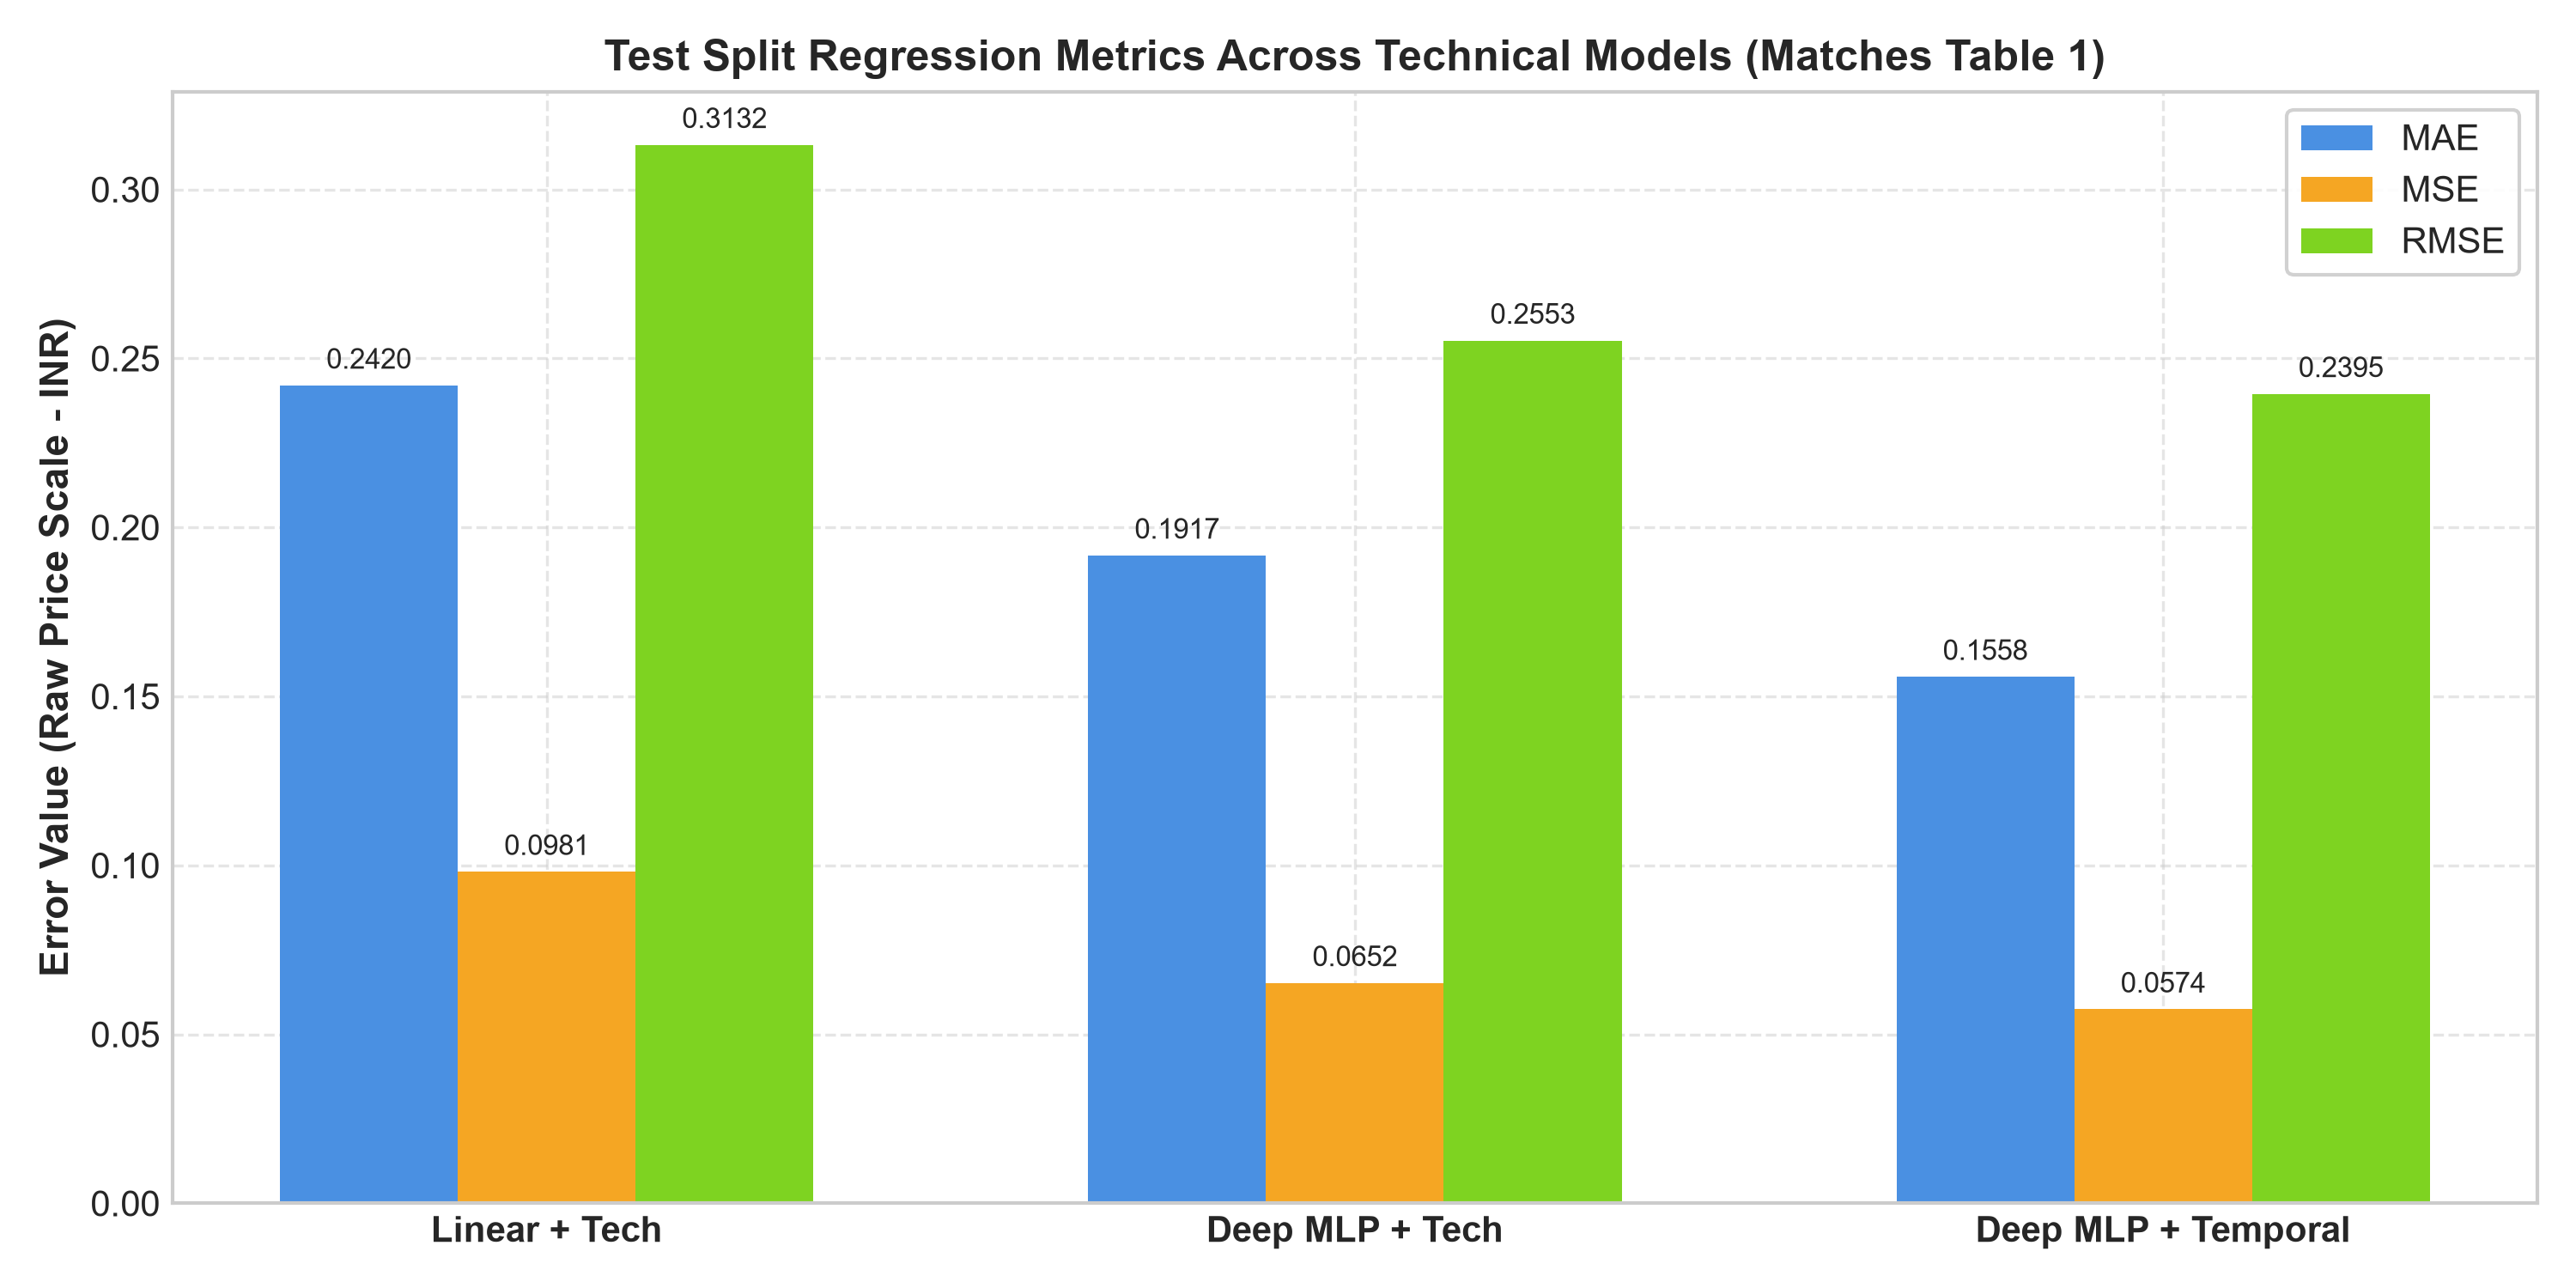
\includegraphics[width=0.8\textwidth]{evaluation-regression-test.png}
		\caption{Test set error breakdown (MAE, MSE, RMSE) across models.}
	\end{figure}
	\begin{itemize}
		\item \textbf{Lowest MAE:} Deep + Technical Indicators achieved \textbf{0.2220} (MAPE 0.25\%).
		\item \textbf{Lowest MSE/RMSE:} Deep + Technical + Temporal achieved \textbf{0.1080} MSE.
	\end{itemize}
\end{frame}

\begin{frame}{Directional Accuracy \& Generalization}
	\begin{figure}[htbp]
		\centering
		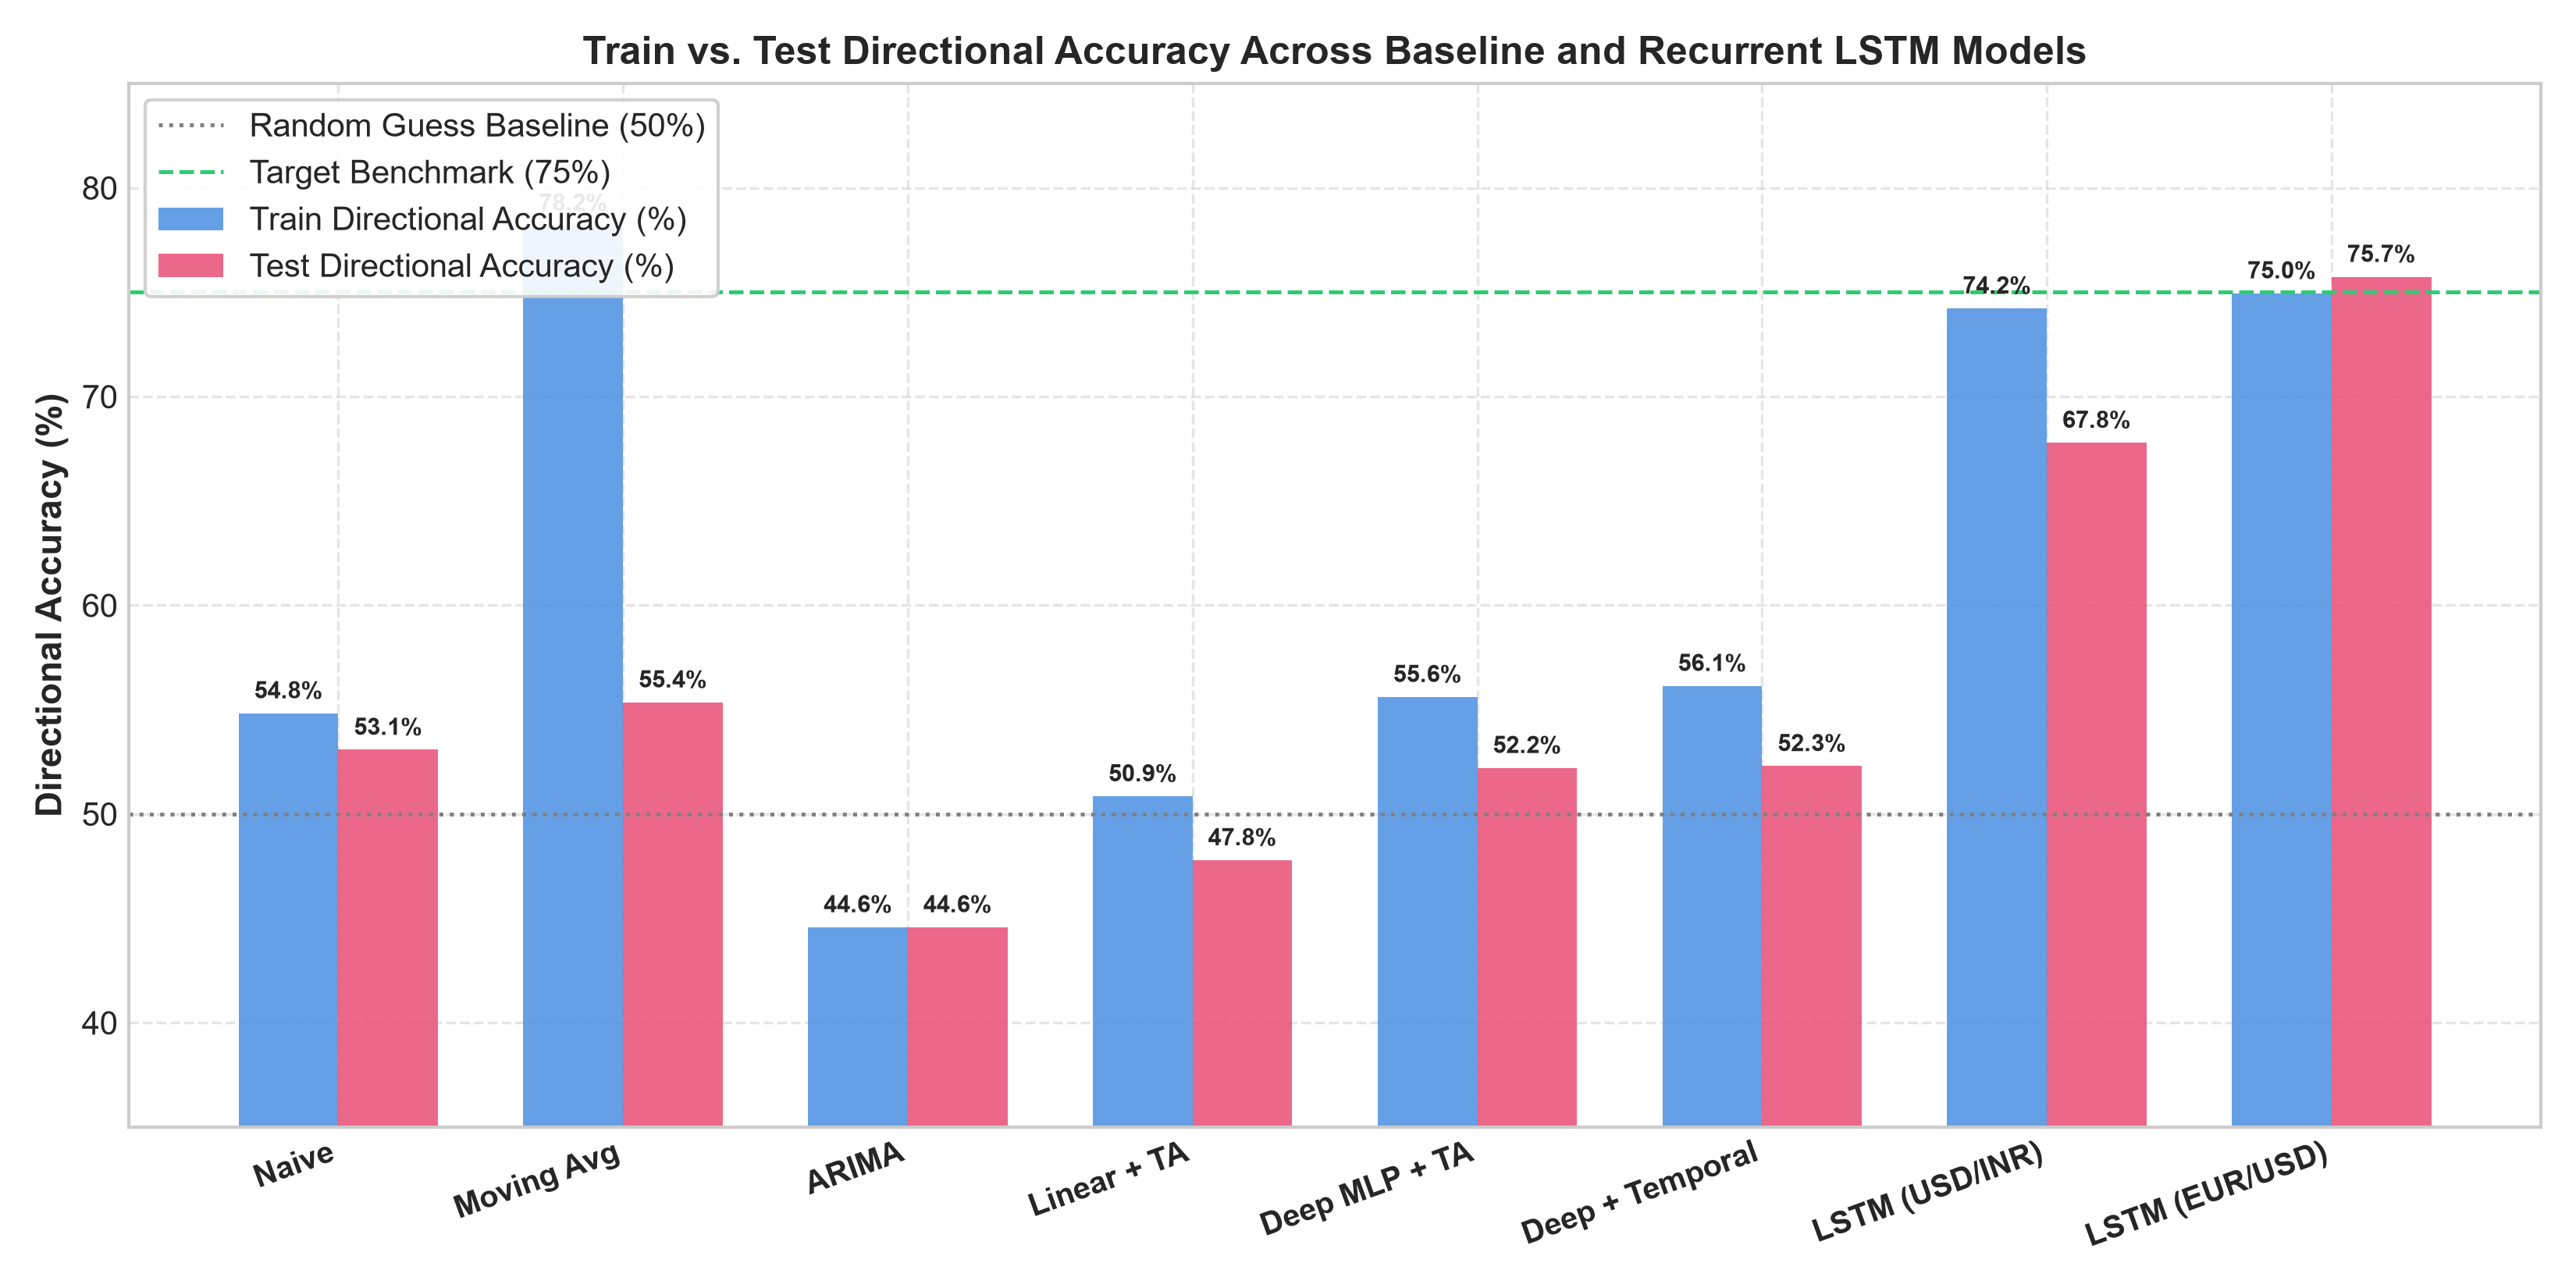
\includegraphics[width=0.8\textwidth]{evaluation-directional-accuracy.png}
		\caption{Comparison of Train vs Test directional accuracy (\%).}
	\end{figure}
\end{frame}

\begin{frame}{Directional Accuracy \& Generalization}
	\begin{itemize}
		\item \textbf{Best Test Directional Accuracy:} Deep + Technical + Temporal reached \textbf{55.85\%}.
	\end{itemize}
\end{frame}

\begin{frame}{Test Set Prediction Tracking}
	\begin{figure}[htbp]
		\centering
		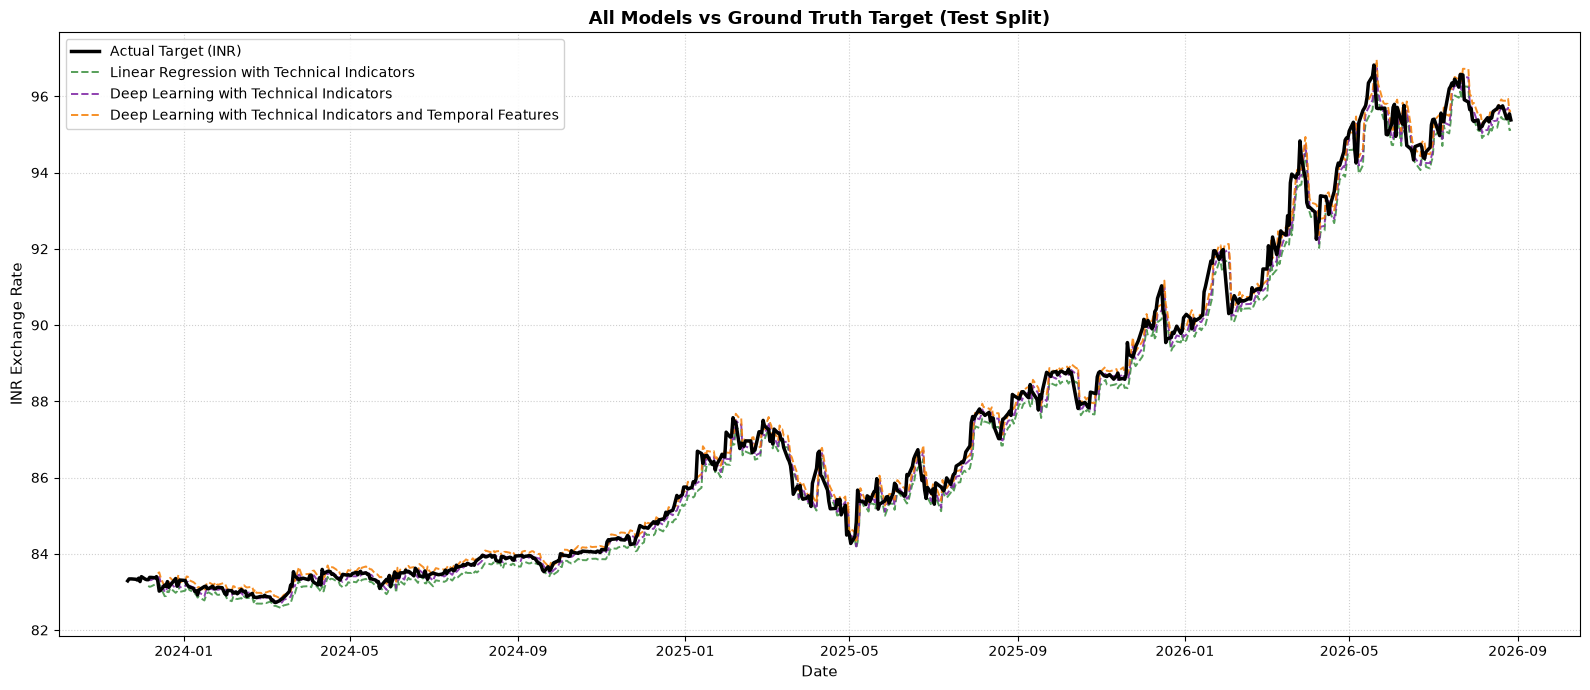
\includegraphics[width=0.85\textwidth]{evaluation-predictions-test.png}
		\caption{Held-out test set predicted trajectories versus actual USD/INR series.}
	\end{figure}
\end{frame}

%========================================================================================
\section{Conclusions \& Proposed Novel Framework}
%========================================================================================
\subsection*{}

\begin{frame}{Proposed Novel Framework: Explainable RL with Macro Differentials}
	\begin{block}{Integrated Architecture for USD/INR Trading}
	\end{block}

	\begin{center}
		\resizebox{\textwidth}{!}{%
		\begin{tabular}{ccccc}
			\textbf{[Macro Differentials + TAs]} & $\longrightarrow$ & \textbf{[GA Feature Selection]} & $\longrightarrow$ & \textbf{[Deep RL Agent (DQN/PPO)]} \\
			& & & & $\downarrow$ \\
			\textbf{[Post-Hoc SHAP Attribution]} & $\longleftarrow$ & \textbf{[Policy Action Execution]} & $\longleftarrow$ & \textbf{[Reward: Risk/Drawdown]} \\
		\end{tabular}%
		}
	\end{center}

	\begin{block}{Key Proposed Innovations}
		\begin{itemize}
			\item \textbf{Macro Differentials Input:} Captures monetary policy divergence ($\Delta y_t$) and market sentiment ($\Delta \text{VIX}_t$).
			\item \textbf{Post-Hoc Policy Attribution:} SHAP value breakdown of $Q(s,a)$ to identify macro triggers behind Buy/Sell/Hold decisions.
		\end{itemize}
	\end{block}
\end{frame}

\begin{frame}{Summary of Key Findings}
	\begin{block}{Core Conclusions}
		\begin{itemize}
			\item \textbf{Technical \& Macro Feature Impact:} Incorporating macro drivers and technical indicators refines representation scale and stability.
			\item \textbf{Temporal Feature Utility:} Adding temporal data paths improves directional hit rate to \textbf{55.85\%} on unseen test data.
			\item \textbf{Validation Integrity:} Chronological splitting prevents data leakage and gives realistic expectations of model performance.
		\end{itemize}
	\end{block}
\end{frame}

\begin{frame}{Future Work \& Next Steps}
	\begin{block}{Planned Research Roadmap}
		\begin{enumerate}
			\item \textbf{Genetic Algorithm Feature Selection:} Optimize macro differential and commodity feature subsets.
			\item \textbf{LSTM Sequence Extension:} Implement 5-lag recurrent LSTM cell for temporal modeling.
			\item \textbf{SHAP Post-Hoc Analysis on RL Agent:} Apply SHAP explainability to Deep Q-Network (DQN) trading policies under macro differential inputs.
			\item \textbf{Walk-Forward Testing \& Cost Simulation:} Incorporate transaction spreads, slippage, and walk-forward validation to bridge predictive accuracy with trade profitability.
		\end{enumerate}
	\end{block}
\end{frame}

\begin{frame}
	\begin{center}
		\Huge \color{iitiblue}\bfseries Thank You!
		
		\vspace{1cm}
		
		\Large Questions \& Discussion
	\end{center}
\end{frame}

\end{document}
